\documentclass[11pt,letterpaper]{article}
\usepackage[T1]{fontenc}
\usepackage[utf8]{inputenc}
\usepackage{lmodern,microtype}
\usepackage[margin=0.92in,headheight=15pt]{geometry}
\usepackage{amsmath,amssymb,amsthm,mathtools}
\usepackage{booktabs,longtable,array,enumitem,graphicx}
\usepackage{xcolor,fancyhdr,xurl}
\usepackage[colorlinks=true,linkcolor=ink,citecolor=teal,urlcolor=teal]{hyperref}
\definecolor{ink}{HTML}{17324D}
\definecolor{teal}{HTML}{087E8B}
\definecolor{muted}{HTML}{526577}
\definecolor{pale}{HTML}{EDF5F7}
\pagestyle{fancy}
\fancyhf{}
\fancyhead[L]{\small\color{muted}Methods beyond Dirichlet GRH}
\fancyhead[R]{\small\color{muted}Research analysis}
\fancyfoot[C]{\thepage}
\setlength{\parskip}{0.45em}
\setlength{\parindent}{0pt}
\setlength{\emergencystretch}{2em}
\newcolumntype{P}[1]{>{\raggedright\arraybackslash}p{#1}}
\setlist[itemize]{leftmargin=1.5em,itemsep=0.2em,topsep=0.3em}
\setlist[enumerate]{leftmargin=1.7em,itemsep=0.3em,topsep=0.3em}
\newtheorem{theorem}{Theorem}[section]
\newtheorem{proposition}[theorem]{Proposition}
\newtheorem{lemma}[theorem]{Lemma}
\newtheorem{corollary}[theorem]{Corollary}
\theoremstyle{remark}
\newtheorem{remark}[theorem]{Remark}
\newcommand{\Q}{\mathbb Q}
\newcommand{\Z}{\mathbb Z}
\newcommand{\R}{\mathbb R}
\newcommand{\C}{\mathbb C}
\newcommand{\N}{\mathbb N}
\newcommand{\Sha}{\mathop{\mathrm{Sha}}\nolimits}
\newcommand{\num}{\operatorname{num}}
\newcommand{\Res}{\operatorname{Res}}
\newcommand{\tr}{\operatorname{tr}}
\newcommand{\length}{\operatorname{length}}
\newcommand{\code}[1]{\texttt{\detokenize{#1}}}
\newcommand{\upstream}{\url{https://github.com/lsernau/grh-lean/tree/72fead102f663d5c7a407964a13dc0cf9d977207}}
\newcommand{\notebox}[1]{\begin{center}\fcolorbox{teal}{pale}{\parbox{0.92\linewidth}{#1}}\end{center}}
\hypersetup{pdftitle={Beyond Dirichlet GRH: averaged zero detection and exact K-theory transfer tests},pdfauthor={Research analysis prepared with ChatGPT}}
\begin{document}
\begin{titlepage}
\vspace*{0.7in}
{\large\color{teal}\bfseries RESEARCH REPORT\par}
\vspace{0.3in}
{\Huge\color{ink}\bfseries Beyond Dirichlet GRH\par}
\vspace{0.2in}
{\LARGE Averaged zero detection and exact\\[4pt]
K-theory transfer tests\par}
\vspace{0.4in}
{\large An analysis of \code{lsernau/grh-lean}\\
and eleven earlier ProveIt reports\par}
\vspace{0.4in}
{\large Prepared for Vladimir Reshetnikov\\
25 November 2026, Pacific date\par}
\vfill
\notebox{\textbf{Principal conclusion.} The internal arithmetic machinery has
credible applications beyond ordinary RH and Dirichlet-GRH consequences.
This report proves two general averaged analytic criteria, gives an exact
arithmetic preparation for the next K-theory degrees, and independently
reconstructs two small Hecke calculations. It proves neither a new
nonabelian RH instance nor a new K-group vanishing theorem.}
\vspace{0.25in}
{\small\color{muted}
Upstream revision: \code{72fead102f663d5c7a407964a13dc0cf9d977207}.\\
ProveIt revision: \code{b65aa6229415bdb66d9ce52decc4e997793cd07d}.\\
All new theorem proofs, exact arithmetic scripts, outputs, source hashes,
and selected source excerpts accompany this report.}
\end{titlepage}
\begingroup
\small
\setlength{\parskip}{0pt}
\tableofcontents
\endgroup
\newpage
\section{Assessment and what this report adds}

The answer to the research question is \textbf{yes, at the level of methods
and identifiable mathematical interfaces}. The source contains arithmetic
constructions and cohomological bounds that have content well beyond its
five final zero-location statements. A particularly concrete application is
the strict-Selmer approach to algebraic K-groups. A second is the prospect of
transporting the determinant argument to Hecke functions over a quadratic
field, and hence to a nonabelian extension of $\Q$.

The new work here is narrower than a claimed resolution of either target.
We derive averaged analytic interfaces that a transferred arithmetic
construction could satisfy, and compute exact preparatory identities for
$K_{124}(\Z)$ and $K_{128}(\Z)$, with a longer screening table through
degree $160$. These additions are accompanied by proofs and reproducible
certificates. Merely repeating the reported $K$-theory application or
listing consequences of Dirichlet GRH would not advance the supplied reports.

\subsection{Exact scope of the repository}

At the pinned revision, both editions export RH and GRH for
\emph{Dirichlet} $L$-functions, all moduli and all characters. The types in
\path{grh/src/Statements.lean} import Mathlib alone; the five corresponding
theorems are in \path{grh/src/Main.lean}. General Hecke functions,
Dedekind zeta functions of arbitrary number fields, and general automorphic
$L$-functions are not additional exported statements \cite{repo}.

The source author reports kernel and comparator checks. More substantially,
Sutherland's independent verification page for this exact revision reports
successful sandboxed builds and independent checker acceptance for both
editions \cite{shortchecks}. We inspected that primary evidence and the
source; we did not repeat the full Lean build or kernel replay in this
investigation. This distinction has no bearing on accepting the user's
premise for the present transfer analysis, but it matters when describing
what this report itself verified.

\subsection{Claim ledger}

\begin{longtable}{@{}P{0.26\linewidth}P{0.42\linewidth}P{0.25\linewidth}@{}}
\toprule
Item & Conclusion & Status here\\
\midrule
\endhead
RH and Dirichlet GRH &
The five upstream statements, at the pinned source revision. &
Imported result; source and external verification examined.\\[5pt]
K-groups through degree $120$ &
Mok--Zheng claim $K_{4m}(\Z)=0$ for $1\le m\le30$. &
Existing follow-on claim; full bridge not independently certified here.\\[5pt]
Positive-part Mellin criterion &
Weighted positive-part integrability excludes all poles in a half-plane. &
Complete human-readable proof in this report.\\[5pt]
Signed moving averages &
An upper bound for every moving interval suffices when the Mellin multiplier
has no zeros in the relevant half-plane. &
Complete proof; sampled signed bins are explicitly distinguished.\\[5pt]
Arithmetic screening through $160$ &
For even $54\le e\le80$, every prime $\ell>109$ admits one of two fields
with three specified Bernoulli values all $\ell$-adic units. &
Exact finite theorem; two independent rational formulas and B\'ezout
certificates.\\[5pt]
Degrees $124$ and $128$ &
The field-selection gcd is $4$ in both cases; dimensions of prospective
comparison spaces are computed. &
Preparation only; no new K-group vanishing.\\[5pt]
Conductor-$23$ nonabelian target &
Three explicit averaged bounds would imply its RH. &
Analytic reductions proved; arithmetic bounds remain open in this work.\\
\bottomrule
\end{longtable}

The analytic arguments are adaptations of classical Landau theory.
The finite rational identities and representation dimensions are claimed
as verified results, without an assertion of bibliographic priority.

\subsection{What the eleven predecessors already contain}

All eleven ZIP archives in the specified incoming directory were downloaded
at the pinned ProveIt revision and checked against their Git blob hashes.
Every manuscript's structure and main claims were read; several relevant
proofs were studied in detail. This is an overlap audit, not a blanket
certification of every theorem in those manuscripts \cite{prior}.

\begin{longtable}{@{}P{0.30\linewidth}P{0.63\linewidth}@{}}
\toprule
Predecessor group & Material already present\\
\midrule
\endhead
Three initial/detailed analysis archives &
The three-input determinant comparison, explicit rank and index losses,
sparse auxiliary twists, the $\Q(\sqrt{-23})$ cubic benchmark, and
K-theory source and quantifier issues.\\[4pt]
Arithmetic and exponent-six archives &
Field classifications and prime representations, nonabelian
one-sided detectors, congruence-prediction obstructions, and
class-group-exponent computations.\\[4pt]
Two CM/prime-bias archives &
Four-term singular-modulus relations, support bounds, Suzuki-type
prime biases, convex balance, and sparse-scale zero tests.\\[4pt]
Newest beyond-Dirichlet archive &
Sharp torsion specialization, integral formal-series extensions,
Fitting-profile control, and comparison of the source's odd cocycles
with an ordinary cohomological local kernel.\\
\bottomrule
\end{longtable}

In particular, the dated analysis already discusses both Pintar and
Mok--Zheng, already proves the product-before-gcd rule, and already
identifies the need to extract a strict-Selmer-to-Hecke theorem. We
attribute those points to the predecessor. Our additional contributions
are the averaged criteria, their precise failure examples, independent
small-operator reconstruction, and exact screening and dimension
calculations beyond the cited $120$ range.

The archive includes a full filename-by-filename audit and provenance
manifest. Some predecessor statements concern new classifications or
large exhaustive computations; they are recorded as predecessor
claims unless separately checked. The present argument does not depend
on those large classifications.

\section{The transferable mechanism in the Lean source}

\subsection{The arithmetic remainder}

For a positive modulus $q$ and an auxiliary prime $d$, the source uses
\[
 R_{d,q}(x)=
 \sum_{\substack{n\le x\\n\equiv1\pmod q}}
 \Lambda(n)(1-\chi_{-d}(n))
       \left(\frac1n-\frac1x\right)
 -\frac{\log x}{\varphi(q)}-c_{d,q}.
\]
Here $\Lambda(p^k)=\log p$ and is zero otherwise. The constant
$c_{d,q}$ centers the expression at infinity. The field and congruence
conditions guarantee that the quadratic character used in the code
agrees with this notation. For example, the final construction takes
$18480\mid q$ and $d\equiv q/2-1\pmod q$.

The smoothing factor $(1/n-1/x)$ is essential. It inserts
$1/[s(s-1)]$ into the Mellin transform, so zero multiplicities appear
with a controlled sign at real points. The source definitions and
transform identities occur in \path{New/Reduction/Zeros/PrimeError.lean};
the place sums that produce this statistic are in
\path{New/Reduction/PrimeSums.lean} \cite{repo}.

\subsection{Three inputs for a common lattice}

The proof constructs spaces of automorphic forms and compares the same
logarithmic squared covolume $V$, corrected by twice an arithmetic index
$\delta$. Its three key inputs are:

\begin{enumerate}
\item \textbf{Short forms.} Theta derivatives yield integral source
forms whose images have controlled size and divisibility.
\item \textbf{Enough forms.} A second-moment argument shows that enough
independent images are present to occupy a large fraction of the target.
\item \textbf{Integral forms are long.} Heights of determinants of
chains of theta lifts, together with the product formula, provide a
lower bound for the same covolume/index expression.
\end{enumerate}

Write $D$ for target dimension, $n$ for the number of independent images,
$H$ for a shared main term, $m$ for chain length, and $\mathrm{rem}$
for the unnormalized prime remainder. Schematically,
\[
 DH-\text{lower loss}
 \ \le\ V+2\delta\
 \le n(H-m\,\mathrm{rem}+\text{upper loss})
       +\text{index loss}.
\]
The main terms cancel. The exact source result is
\[
 m\,\mathrm{rem}\le f\,a(\log b)^5.
\]
After converting the place sum to $R_{d,q}$, a further factor of
$\log b$ appears. With $m\ge\sqrt x$, $\log b\le2x^\varepsilon$,
and errors controlled at a much larger cutoff $x_1$, the source proves
\[
 R_{d,q}(x)\le(64\varphi(q)+3)x^{-1/2+6\varepsilon}
\]
for large integers $x$. Interpolation and adjustment of $\varepsilon$
give the final all-real-scale one-sided bound
\cite{mainineq,onesided}.

This square-root amplification is a specific arithmetic accomplishment.
Introducing a symbol $m=\sqrt x$ in an unrelated problem would not
reproduce it: the shortness, integrality, spanning, denominator, and
determinant-height estimates must all hold at that chain length.

\subsection{Two distinct uses of twisting}

Twists serve two separate purposes. Inside the arithmetic argument they
control local denominators and compare determinant heights; a good
twist may be selected separately at each coefficient prime. In the
analytic endgame an auxiliary quadratic twist is selected to avoid
zeros in a prescribed rectangle.

The latter is necessary because the transformed remainder detects a
\emph{difference} of zero-multiplicity sums. A zero of an untwisted
function could be canceled by a twisted zero at the same point.
The source's zero-density input selects a $d$ for which the twisted
terms have no zeros in the relevant box. The residual numerator is
then a sum of nonnegative integers. Landau's positivity argument
converts the one-sided upper bound into pole exclusion
\cite{criterion}.

For a full Dedekind-zeta statistic, zero multiplicities can instead
already have the same sign. That removes the auxiliary analytic
zero-avoidance step. It does not remove any twists still needed by
the arithmetic construction.

\subsection{What can be transported and what must be rebuilt}

The scalar determinant comparison, the product-formula logic, and the
Landau transform argument admit clean general statements. In contrast,
the construction of the prime weights and the sufficient supply of
forms are specific to the chosen CM field, level, local types, and
theta chain.

For a new $L$-function, the central design question is therefore:
\emph{which arithmetic object produces its actual prime or prime-ideal
coefficients, with the correct normalization and controlled losses?}
An appealing analogy to theta lifting is insufficient without that
coefficient identity.

The next section changes the analytic interface. It shows that a
successful new arithmetic construction need not necessarily give an
estimate at every individual scale. Suitable averages can supply all
the analytic information needed.

\section{A transfer criterion requiring only positive error in mean}
\label{sec:mean-transfer}

This section gives a self-contained strengthening of the analytic interface used in
the repository.  It does not establish a new zero-free region for a new
$L$-function: the arithmetic estimate in the application below remains to be
proved.  The contribution relative to the incoming reports is to replace the
pointwise arithmetic target by a positive-part estimate in mean, and to state
exactly how nonuniform rank and denominator losses can feed that estimate.
The analytic argument is an adaptation of classical Landau theory, not a claim
that the underlying analytic principle is new to the literature.

For a real number $u$, write $u_+=\max(u,0)$ and $u_-=\max(-u,0)$.

\begin{theorem}[Positive-part Mellin criterion]\label{thm:positive-mellin}
Let $\beta>0$, and let $R:[1,\infty)\to\mathbb R$ be measurable and locally
integrable, with $|R(x)|\le Cx^A$ for all sufficiently large $x$, for some
finite constants $A,C$. Suppose
\[
 F(s)=\int_1^\infty R(x)x^{-s}\,dx
\]
initially defined for $\Re s>A+1$, has a meromorphic continuation to
$\Re s>\beta$ with at most simple poles.  At every real $u>\beta$, suppose
the residue of $F$ is a nonnegative real number, with residue zero at a
regular point.  If
\begin{equation}\label{eq:positive-integrability}
 \int_1^\infty R(x)_+x^{-\sigma}\,dx<\infty
 \qquad\hbox{for every real }\sigma>\beta,
\end{equation}
then $F$ is holomorphic throughout $\Re s>\beta$. Moreover
\[
 \int_1^\infty |R(x)|x^{-\sigma}\,dx<\infty
 \qquad(\sigma>\beta).
\]
\end{theorem}

\begin{proof}
Put $H(s)=\int_1^\infty R(x)_+x^{-s}\,dx$. Condition
\eqref{eq:positive-integrability}, with a slightly smaller real exponent to
dominate derivatives, makes $H$ holomorphic on $\Re s>\beta$. Far to the
right,
\[
 G(s):=H(s)-F(s)=\int_1^\infty R(x)_-x^{-s}\,dx.
\]
The right-hand side is the Mellin transform of a nonnegative function. Let
$a\in[-\infty,\infty)$ be its abscissa of convergence; the polynomial growth
hypothesis makes $a$ bounded above. It is enough to prove $a\le\beta$.

Suppose $a>\beta$. The meromorphic function $H-F$ continues $G$ to a
neighborhood of $a$. It agrees with $G$ in $\Re s>a$ by the identity theorem.
Its residue at $a$ equals $-\operatorname{Res}_{s=a}F(s)\le0$. On the other
hand, $G(\sigma)\ge0$ for real $\sigma>a$, so
\[
 \operatorname{Res}_{s=a}(H-F)
 =\lim_{\sigma\downarrow a}(\sigma-a)G(\sigma)\ge0.
\]
Thus the residue is zero. Because the possible pole is at most simple,
$H-F$ is holomorphic at $a$. This contradicts Landau's theorem: a Mellin
transform of a nonnegative locally integrable function, equivalently its
Laplace transform after $x=e^v$, cannot be holomorphic at its finite abscissa
of convergence. Hence $a\le\beta$.

Both positive and negative parts now have absolutely convergent transforms
for every real $\sigma>\beta$. Their difference is holomorphic there and,
by analytic continuation, equals $F$. Their sum proves the final assertion.
\end{proof}

The exact source interface for the Landau step is
\path{Lib/Analytic/Landau.lean}, especially
\path{exists_Ioi_subset_integrableExpSet_of_analyticAt}
(lines 160--176) and
\path{exists_Ioi_subset_integrableExpSet}
(lines 182--210) at the pinned commit.  The repository's
\texttt{IsPolar.landau} (lines 217--259) instead subtracts a fixed
exponential majorant. The present proof subtracts the holomorphic transform
of the whole positive part \cite{landau}.

\begin{corollary}[Dyadic and square-mean versions]\label{cor:mean-versions}
Under the analytic hypotheses of Theorem~\ref{thm:positive-mellin}, either
of the following conditions suffices to exclude all poles with $\Re s>\beta$:
\begin{align}
 \int_X^{2X}R(x)_+\,dx&\ll_\varepsilon X^{\beta+\varepsilon},
       &&\hbox{for every }\varepsilon>0,\label{eq:mean-lone}\\
 \int_X^{2X}R(x)_+^2\,dx&\ll_\varepsilon X^{2\beta-1+\varepsilon},
       &&\hbox{for every }\varepsilon>0.\label{eq:mean-ltwo}
\end{align}
Here it is enough that the estimates hold for all sufficiently large
dyadic $X=2^k$. In fact \eqref{eq:mean-lone} is equivalent to
\eqref{eq:positive-integrability}.
\end{corollary}

\begin{proof}
For $\sigma>\beta$, choose $0<\varepsilon<\sigma-\beta$ and sum
\[
 \int_{2^k}^{2^{k+1}} R(x)_+x^{-\sigma}\,dx
 \ll_\varepsilon 2^{k(\beta+\varepsilon-\sigma)}.
\]
The geometric series converges. Conversely, integrability at
$\sigma=\beta+\varepsilon$ bounds a dyadic block by a constant times
$X^{\beta+\varepsilon}$. Finally Cauchy--Schwarz gives
\[
 \int_X^{2X}R(x)_+\,dx
 \le X^{1/2}\left(\int_X^{2X}R(x)_+^2\,dx\right)^{1/2},
\]
which takes \eqref{eq:mean-ltwo} to \eqref{eq:mean-lone}.
\end{proof}

The integral condition really allows positive spikes that no eventual
pointwise bound allows. For example, let $R$ be the indicator of the disjoint
intervals $[2^k,2^k+2^{-2k}]$, $k\ge1$. Its Mellin transform is holomorphic
on $\Re s>-2$, and its positive part satisfies the criterion for
$\beta=1/2$, but $R(x)\le x^{-1/2+\varepsilon}$ fails arbitrarily far out
for every $0<\varepsilon<1/2$.

\subsection{An exact averaged determinant certificate}

The source proof compares a lower bound on the same covolume plus twice an
index with an upper bound obtained from many short vectors. Its scalar
content can be retained while allowing the fraction of available vectors to
vary strongly with $x$.
The scalar rearrangement already appears in the predecessors; its use
below with an averaged inverse-rank loss is the additional interface.

\begin{proposition}[Rank-sensitive loss]\label{prop:rank-loss}
At each $x$ suppose $d>0$, $0<n\le d$, $M>0$, $H\ge0$, and $L,U,I\ge0$.
Suppose a real number $V$ satisfies
\[
 d(H-L)\le V+2dI,
 \qquad
 V\le n\bigl(H-MR(x)+U\bigr).
\]
Writing $\alpha=n/d$, one has the exact scalar implication
\begin{align}
 R(x)_+
 &\le\frac{\bigl(L+\alpha U+2I-(1-\alpha)H\bigr)_+}{\alpha M}
 \label{eq:rank-exact}\\
 &\le\frac{1}{M}\left(U+\frac{L+2I}{\alpha}\right).
 \label{eq:rank-coarse}
\end{align}
\end{proposition}

\begin{proof}
Combine the two inequalities, divide by $d$, and rearrange to obtain
\[
 \alpha M R(x)\le L+\alpha U+2I-(1-\alpha)H.
\]
Taking positive parts and dividing by $\alpha M>0$ proves
\eqref{eq:rank-exact}. Since $H\ge0$, $\alpha\le1$, and
$L+\alpha U+2I\ge0$, dropping the nonpositive term gives
\eqref{eq:rank-coarse}.
\end{proof}

Thus one must first combine the bounds for each $x$, and then average the
combined loss. Let
\[
 A(x)=U(x)+\frac{L(x)+2I(x)}{\alpha(x)}.
\]
If $M(x)\ge c x^\theta$ with $0<\theta<1$, and for every
$\varepsilon>0$
\begin{equation}\label{eq:mean-arithmetic-target}
 \int_X^{2X} A(x)\,dx\ll_\varepsilon X^{1+\varepsilon},
\end{equation}
then \eqref{eq:rank-coarse} implies
\[
 \int_X^{2X}R(x)_+\,dx
 \ll_\varepsilon X^{1-\theta+\varepsilon}.
\]
If $R$ has the analytic properties of Theorem~\ref{thm:positive-mellin},
this excludes poles with $\Re s>1-\theta$. The factor $M$ may itself
be a product of the number of lifts and the normalization of the prime
statistic; keeping that normalization is essential when applying the formula.

There is no requirement of a uniform positive lower bound for $\alpha$.
For example, conjugate exponents $p,q>1$ with $1/p+1/q=1$ give the
sufficient conditions
\begin{align*}
 \int_X^{2X}U(x)\,dx&\ll_\varepsilon X^{1+\varepsilon},\\
 \int_X^{2X}(L(x)+2I(x))^p\,dx&\ll_\varepsilon X^{1+\varepsilon},\\
 \int_X^{2X}\alpha(x)^{-q}\,dx&\ll_\varepsilon X^{1+\varepsilon}.
\end{align*}
H\"older's inequality proves \eqref{eq:mean-arithmetic-target}. The
case $p=q=2$ gives a particularly concrete square-mean test. Bounding
the averages of $L,I,\alpha$ separately is insufficient: on a probability
space, let $L=1$, and let $\alpha=\delta^2$ with probability $\delta$
and $\alpha=1$ otherwise. Then $\mathbb E L=1$ and
$\mathbb E\alpha=1-\delta+\delta^3\to1$, but
$\mathbb E(L/\alpha)=1-\delta+\delta^{-1}\to\infty$.

\subsection{Application to the nonabelian cubic target}

Let $K=\mathbb Q(\sqrt{-23})$, let $H$ be its Hilbert class field, and
let $\mathcal R_H$ be the earlier report's principal-ideal remainder
\[
 \mathcal R_H(x)=
 3\sum_{\substack{N\mathfrak a\le x\\{}[\mathfrak a]=1}}
 \Lambda_K(\mathfrak a)\left(\frac1{N\mathfrak a}-\frac1x\right)
 -\log x+1+\gamma_H.
\]
Its Mellin transform is
\[
 \frac{-\zeta_H'(s)/\zeta_H(s)}{s(s-1)}
 -\frac1{(s-1)^2}+\frac{1+\gamma_H}{s-1}.
\]
The singularity at $s=1$ is removable. A nontrivial zero $\rho$ of
multiplicity $m_\rho$ gives residue
$m_\rho/[\rho(1-\rho)]$, which is nonnegative at real
$0<\rho<1$. The coefficient bound
$0\le\Lambda_H(n)\le6\Lambda(n)$ gives the required elementary growth.
Consequently either one of
\begin{align*}
 \int_X^{2X}\mathcal R_H(x)_+\,dx
    &\ll_\varepsilon X^{1/2+\varepsilon},\\
 \int_X^{2X}\mathcal R_H(x)_+^2\,dx
    &\ll_\varepsilon X^\varepsilon
\end{align*}
for every $\varepsilon>0$ would prove RH for $\zeta_H$ and hence for the
degree-two class-character $L$-function and the cubic Dedekind zeta function.
These require a weaker form of arithmetic control than the earlier eventual
pointwise bound; for this fixed remainder, successful control would still
be equivalent to the same zero-location assertion. They remain unproved here. The new calculation identifies what an
arithmetic construction in mean would have to deliver; it does not supply
that construction.

\subsection{Signed moving averages also suffice, if every starting point is controlled}

There is a different useful relaxation in which cancellation is allowed but
the starting point of the averaging interval must vary continuously. This
must be distinguished from checking only the fixed dyadic partition.

\begin{theorem}[Signed moving-window criterion]\label{thm:moving-window}
Assume the analytic hypotheses of Theorem~\ref{thm:positive-mellin}, and
fix $h>1$. If, for some $C\ge0$,
\begin{equation}\label{eq:moving-signed}
 \int_x^{hx}R(t)\,dt\le Cx^\beta
 \qquad\hbox{for every sufficiently large real }x,
\end{equation}
then $F$ is holomorphic in $\Re s>\beta$.
It also suffices, for a desired boundary $\beta$, to prove
\eqref{eq:moving-signed} with exponent $\beta+\varepsilon$ for every
$\varepsilon>0$, with constants allowed to depend on $\varepsilon$.
\end{theorem}

\begin{proof}
Set $T_hR(x)=x^{-1}\int_x^{hx}R(t)\,dt$. Fubini's theorem, initially
far to the right, gives
\begin{align*}
 F_{T_hR}(s)
 &=\frac{h^s-1}{s}F(s)
 -\frac1s\int_1^h R(t)\bigl(h^s t^{-s}-1\bigr)\,dt.
\end{align*}
Indeed the inner integral in the reversed order is
$\int_{\max(1,t/h)}^t x^{-s-1}\,dx$; splitting the outer integral
at $t=h$ proves the formula. The finite-interval correction is entire:
the apparent singularity at $s=0$ is removable. The multiplier
$A_h(s)=(h^s-1)/s$ is entire, is nonzero on $\Re s>0$, and is
strictly positive for real $s>0$. Thus the poles of $F_{T_hR}$ in
$\Re s>\beta$ have exactly the poles of $F$, and their real residues
are nonnegative.

The estimate \eqref{eq:moving-signed} gives
$T_hR(x)\le Cx^{\beta-1}$ eventually. Since $R$ is locally integrable,
$T_hR$ is continuous and bounded on each compact interval. Enlarge $C$ to
$K$ so that $Kx^{\beta-1}-T_hR(x)\ge0$ for all $x\ge1$.
Its transform is
$K/(s-\beta)-F_{T_hR}(s)$. At real points greater than $\beta$
its residues are nonpositive. The same Landau abscissa argument as above
therefore shows that $F_{T_hR}$ has no pole to the right of $\beta$.
Since $A_h$ has no zero there, neither does $F$ have a pole. Apply the
fixed-exponent result for each $\beta+\varepsilon$ to get the last claim.
\end{proof}

In particular, for the cubic-field target one may instead aim for
$\int_x^{2x}\mathcal R_H(t)\,dt\le C_\varepsilon
x^{1/2+\varepsilon}$ for \emph{every} sufficiently large real $x$.
This allows signed cancellation.  No corresponding arithmetic estimate is
proved here. The positive-part criterion is more robust when the available
information is restricted to the sampled dyadic intervals.

\subsection{Why signed averages on the dyadic grid are insufficient}

The positive part in the criterion cannot simply be removed. Fix
$0<\beta<a<1$, put $\tau=2\pi/\log2$, and set
\[
 R(x)=\frac{d}{dx}\bigl(x^a\sin(\tau\log x)\bigr)
 =x^{a-1}\bigl(a\sin(\tau\log x)+\tau\cos(\tau\log x)\bigr).
\]
For every integer $k\ge0$,
\[
 \int_{2^k}^{2^{k+1}}R(x)\,dx=0.
\]
Nevertheless
\[
 F(s)=\int_1^\infty R(x)x^{-s}\,dx
 =\frac{\tau s}{(s-a)^2+\tau^2}
 \qquad(\Re s>a),
\]
which has nonzero simple poles at $a\pm i\tau$, to the right of
$\beta$, and no real poles. All other analytic hypotheses of
Theorem~\ref{thm:positive-mellin} hold. Moreover
\[
 \int_{2^k}^{2^{k+1}}R(x)_+\,dx=C_a\,2^{ka}
 \quad\hbox{with }C_a>0.
\]
This follows by substituting $x=2^k e^u$, $0\le u\le\log2$.
Thus cancellation in signed bin averages can hide precisely the poles
that the arithmetic transfer is intended to exclude. This example concerns
signed averages on the fixed dyadic partition; it does not assert failure of
every translated smoothing condition.

\section{What the averaged criteria do and do not permit}

\subsection{The cubic normalization and the precise new target}

For clarity, here is the full normalization used in the application.
Let $H$ be the splitting field of $X^3-X-1$. This is the Hilbert
class field of $K=\Q(\sqrt{-23})$, whose class group has order $3$.
If $\psi$ is a nontrivial ideal-class character of $K$ and
$F=\Q(\theta)$ for a root $\theta$, then
\[
 \zeta_F(s)=\zeta(s)L_K(s,\psi),\qquad
 \zeta_H(s)=\zeta(s)L(s,\chi_{-23})L_K(s,\psi)^2.
\]
These are the exact factorization identities established and referenced
in the predecessor's cubic benchmark \cite{priorcubic}.
The degree-two factor is a Hecke function over $K$; it is not a
Dirichlet $L$-function over $\Q$.

Define the normalized Euler--Kronecker constant by
\[
 \zeta_H(s)=\frac{\kappa_H}{s-1}
              +\kappa_H\gamma_H+O(s-1).
\]
If $-\zeta_H'/\zeta_H=\sum a_H(n)n^{-s}$, its coefficients obey
$0\le a_H(n)\le6\Lambda(n)$ and
\[
 a_H(n)=3\!\!\sum_{\substack{N\mathfrak a=n\\{}[\mathfrak a]=1}}
                 \Lambda_K(\mathfrak a).
\]
The identity follows by summing the three class characters; character
orthogonality keeps exactly the principal ideal powers. Thus the
statistic in the previous section is also
\[
 \mathcal R_H(x)=
 \sum_{n\le x}a_H(n)\left(\frac1n-\frac1x\right)
       -\log x+\gamma_H+1.
\]

Writing $z=s-1$, direct multiplication gives
\[
 \frac{-\zeta_H'(s)/\zeta_H(s)}{s(s-1)}
   =z^{-2}-(\gamma_H+1)z^{-1}+O(1).
\]
This verifies both subtractions at $s=1$.
At a zero $\rho$ of multiplicity $m_\rho$, the residue is
$m_\rho/[\rho(1-\rho)]$. On the real part of the critical strip it
is positive; beyond $1$ there are no zeros. Therefore the
positive-part and moving-average theorems apply without a
zero-avoiding auxiliary analytic twist.

There are now three concrete targets, each sufficient:
\[
\boxed{\begin{aligned}
 &\int_X^{2X}(\mathcal R_H)_+\,dx
        \ll_\varepsilon X^{1/2+\varepsilon}
        &&\text{on dyadic }X;\\
 &\int_X^{2X}(\mathcal R_H)_+^2\,dx
        \ll_\varepsilon X^\varepsilon
        &&\text{on dyadic }X;\\
 &\int_X^{2X}\mathcal R_H\,dx
        \le C_\varepsilon X^{1/2+\varepsilon}
        &&\text{for all large real }X.
\end{aligned}}
\]
Every statement is for all $\varepsilon>0$. The third is genuinely
one-sided; replacing its inequality by absolute-value big-$O$
notation would unnecessarily strengthen it.

None is proved arithmetically here. A successful estimate would
settle a nonabelian RH instance, and would do so using information
beyond the source's Dirichlet factors. Conversely, this fixed field's
RH supplies conventional smoothed error bounds and hence these
averaged bounds. The distinction is a weaker \emph{form of control
to aim for}, not a claim of a conjecture logically weaker than that
RH instance.

For this statistic, the elementary bound
$|\mathcal R_H(x)|=O_H(\log^2(2x))$ also means that integer starting
points suffice for the third target: changing $X$ by at most one
changes the two endpoints by bounded amounts and costs only
$O_H(\log^2(2X))$ in the unnormalized integral. This observation
does not permit exponentially sparse starting points.

\subsection{A continuous example separating average and pointwise control}

The relaxation remains real even if a function tends to zero and
varies slowly. For each $X=2^k$, put a triangular bump at $3X/2$,
of height $X^{-1/4}$ and half-width $X^{3/4}/4$, and set $R$ to
zero between these bumps. The supports are disjoint and lie within
their respective dyadic bins. Exact triangle areas give
\[
 \int_X^{2X}R(x)_+\,dx=\frac14X^{1/2},
 \qquad |R'(x)|\le\frac7x
 \quad\text{where the derivative exists}.
\]
The function is continuous and tends to zero. Its Mellin integral
converges absolutely, and defines a holomorphic function, throughout
$\Re s>1/2$. Nevertheless, at the bump centers,
\[
 R(3X/2)=X^{-1/4},
\]
which is not $O(x^{-1/2+\varepsilon})$ for any
$0<\varepsilon<1/4$. Thus the positive-part mean criterion does
not hide an equivalent pointwise assumption on general functions.

\begin{figure}[htbp]
\centering
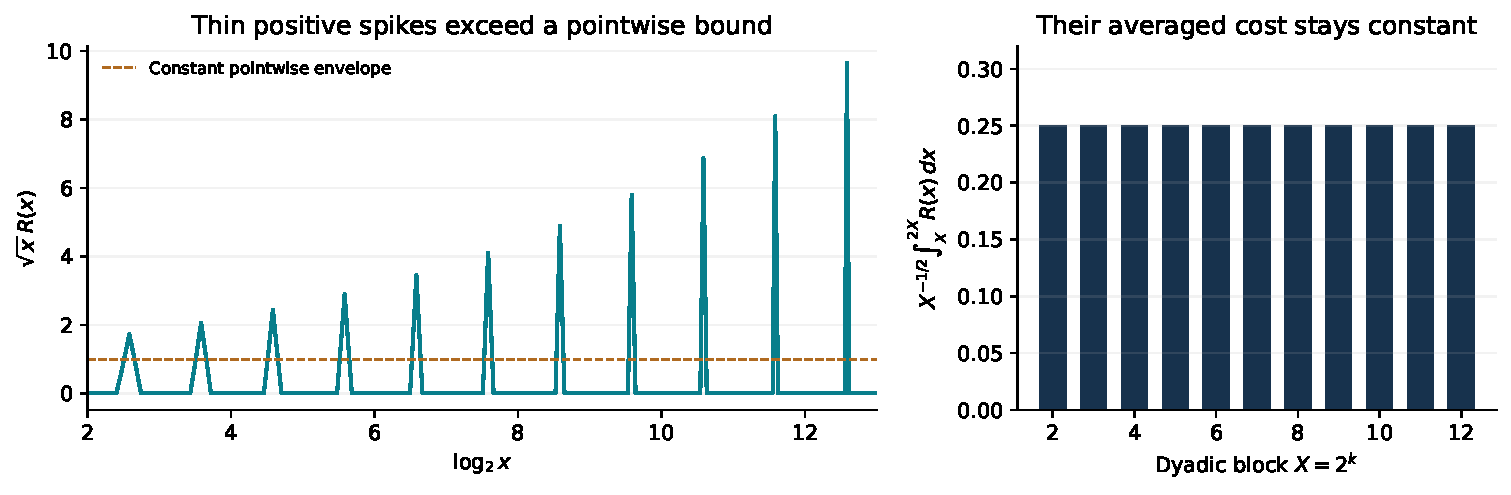
\includegraphics[width=\linewidth]{figures/averaged_spikes.pdf}
\caption{A synthetic exact model, not prime data. The normalized
pointwise peaks grow, while every normalized dyadic positive area is
$1/4$. The mathematical identities are checked with rational
arithmetic; floating point is used only to draw the figure.}
\end{figure}

\subsection{Two further analytic checks}

\textbf{The sign and real-pole hypothesis cannot be omitted.}
For $\beta<a<1$, the function $R(x)=-x^{a-1}$ has
$R_+=0$, yet $F(s)=-1/(s-a)$ has a real pole of negative residue.
Likewise $R(x)=-x^{a-1}\log x$ gives
$F(s)=-1/(s-a)^2$: its residue is zero, but it has a double real
pole. In fact the theorem needs simplicity only at real poles;
nonreal poles may have arbitrary finite order.

\textbf{A positive averaging kernel can still conceal poles.}
It is essential that the moving-box multiplier has no zeros in
the desired half-plane. Set
\[
 R(x)=x^{a-1}\cos\!\left(\frac{\pi\log x}{\log2}\right),
 \qquad \beta<a<1.
\]
Then the positive weighted combination
\[
 R(x)+2^{1-a}R(2x)=0
\]
vanishes identically, while the Mellin transform of $R$ has poles
at $a\pm i\pi/\log2$. Positivity of averaging weights alone is
insufficient. The explicit zero-free multiplier
$(h^s-1)/s$ is what makes the moving-box theorem valid.

There is also a useful weighted-box variant. For real $\nu$, set
\[
 T_{h,\nu}R(x)=x^{-1-\nu}\int_x^{hx}t^\nu R(t)\,dt.
\]
The same calculation yields multiplier
$(h^{s+\nu}-1)/(s+\nu)$, whose zeros lie on
$\Re s=-\nu$. Thus the moving criterion remains valid on
$\Re s>\beta$ whenever $\beta+\nu\ge0$. This can accommodate
a power normalization arising naturally from an averaged
determinant calculation. For an arbitrary varying weight, the
transform must be checked afresh.

\section{The K-theory transfer: source distinctions and new exact tests}
\label{sec:ktheory}

\subsection{Why this is beyond a usual RH consequence}

The groups $K_{4m}(\Z)$ encode higher algebraic information about the
integers. Their proposed vanishing is connected to cyclotomic class groups
and strict Galois-cohomology groups. A bound on one of those groups inside
the original RH proof can therefore have an application that does not
factor through the final assertion about zeta zeros.

Mok--Zheng's November 24 preprint claims
\[
 K_{4m}(\Z)=0\qquad(1\le m\le30).
\]
Pintar's current preprint states a conditional range through degree $104$,
retaining the original Step 17 arithmetic construction as a hypothesis.
The former reports that its modified Gaussian Lean entry point has not
been fully rebuilt; the latter invokes a common-representation extraction
from a separate research archive. These are different proof routes and
different verification statuses \cite{mokzheng,pintar}.

The earlier ProveIt analysis already recognized these developments.
The useful new work is to expose the interfaces and test arithmetic
beyond the published ranges, while keeping the unverified logical
steps visible.

\subsection{The short repository does not export the required strict bound}

The current short source proves
\path{New.exists_length_shaOdd_le}. For a fixed cyclotomic CM field
$E\subseteq\Q(\mu_N)$ and a fixed range of Tate exponents, it supplies
one nonzero integer whose valuations bound lengths of certain odd
cocycle modules. Its documentation explicitly distinguishes that
model from ordinary $\Sha^1$ \cite{oddsha}.

The newest predecessor supplies a comparison with an ordinary local
cohomology kernel, for odd coefficient primes and positive Tate
exponents. Its conjugation eigenspace is
\[
 \Sha^1(E,(F/\mathcal O)(-e))^{c=(-1)^{e+1}}.
\]
For even $e$, this is the natural minus eigenspace. Rational classes
needed in the direct $K_{4m}(\Z)$ route lie in the natural plus
eigenspace after restriction. A length bound on the former is not a
vanishing theorem for the latter. Also, an integer obtained after
fixing $E$ cannot be used uniformly after replacing $E$ by
$\Q(\mu_\ell)$ as $\ell$ varies \cite{priorbeyond}.

The original interface used by the K-theory papers is instead
\path{UpperTheory.V.Z.J.OneCharU_s}, in the much larger original
development, with the caller \path{SmallClassNumbers/CorGKOf.lean}.
Those names are absent from the shorter source tree. We inspected
the original definitions at the separately pinned mirror revision
\code{7cbf7a0c32fca1badf05931879a37c3f8a2b03b4}
\cite{originalinterface}.

In the pointwise formulation, a Galois element is selected first;
the finite family of admissible automorphic witnesses may depend
on that element. Pintar's stronger route extracts a common
representation from the construction behind the inequality.
The inequality alone does not exchange these quantifiers.

There is a further concrete field issue. For the original parameters
$N=2$, an even exponent, and trivial character, the fields
$\Q(\sqrt{-3})$ and $\Q(\sqrt{-7})$ satisfy the relevant
odd-discriminant coprimality condition. The Gaussian field $\Q(i)$
does not: $\gcd(4,2)\ne1$. Using it therefore requires the additional
proof transfer described by Mok--Zheng, rather than substitution
into the unmodified original hypothesis.

\subsection{How to aggregate finite certificates correctly}

For a finite set of valid Frobenius probes $q$, suppose a nonzero
Selmer group forces at least one of the integral branch determinants
$A_{qj}$ to be divisible by a coefficient prime $\ell$.
Then
\[
 \bigl(\forall q\ \exists j:\ell\mid A_{qj}\bigr)
 \quad\Longleftrightarrow\quad
 \ell\mid\gcd_q\prod_j A_{qj}.
\]
This is the product-before-gcd rule already proved in the dated
predecessor. Validity of the probe, integrality of the chosen lattice,
and the target trace normalization are hypotheses of the
divisibility statement, not consequences of the integer calculation.

There is an additional useful refinement for \emph{stronger} inputs.

\begin{proposition}[Exact certificate for alternative length bounds]
\label{prop:lcm}
Let the probe set and each corresponding branch set be finite and
nonempty. Let $A_{qj}$ be nonzero integers, and suppose a nonnegative integer
$r_\ell$ satisfies
\[
 \forall q\ \exists j:\quad r_\ell\le v_\ell(A_{qj}).
\]
Set
\[
 C=\gcd_q\operatorname{lcm}_j|A_{qj}|.
\]
Then
\[
 r_\ell\le v_\ell(C)
       =\min_q\max_jv_\ell(A_{qj}).
\]
The right side is the largest bound permitted by these numerical
inequalities alone.
\end{proposition}

\begin{proof}
At a fixed probe the existence of a branch is equivalent to
$r_\ell\le\max_jv_\ell(A_{qj})$. Intersecting the bounds over probes
takes the minimum. Prime valuations turn lcm into maximum and gcd
into minimum. Taking $r_\ell$ equal to that minimum demonstrates
sharpness as a statement about the numerical hypotheses.
\end{proof}

If $r_\ell$ is the length of a finite $\Z_\ell$-module, its
$\ell$-primary exponent is consequently at most $\ell^{v_\ell(C)}$.
This conclusion requires the displayed length hypothesis. The
mere nonzero-witness condition imposes no such bound: for rows
$(2,3)$ and $(3,2)$, the prime $2$ survives all probes regardless
of whether the module is $\Z/2\Z$ or $\Z/2^{100}\Z$.

If the genuine source estimate is a \emph{sum} of valuations of
simultaneous witnesses, products are still needed. The lcm
refinement must not be silently applied to Mok--Zheng's valuation
sum. It describes a precise improvement available only after a
stronger branchwise length theorem has been established.

\subsection{A finite arithmetic theorem beyond the cited degree range}

For $d\in\{3,7\}$ let $\chi_{-d}(a)=(a/d)$, an odd quadratic
Dirichlet character. Define generalized Bernoulli numbers by
\[
 \sum_{m\ge0}B_{m,\chi_{-d}}\frac{t^m}{m!}
 =\frac{t\sum_{a=1}^{d-1}\chi_{-d}(a)e^{at}}{e^{dt}-1},
\]
and put
\[
 b_d(n)=\frac{B_{n+1,\chi_{-d}}}{n+1},\qquad
 A_d(e)=\left|\num b_d(e)\,\num b_d(2e)\right|.
\]
Numerators and denominators are always reduced to lowest terms.

\begin{theorem}[Exact two-field unit screening]\label{thm:screening}
For every even $e$ with $54\le e\le80$ and every prime $\ell>109$,
there is $d\in\{3,7\}$ for which
\[
 b_d(0),\quad b_d(e),\quad b_d(2e)
\]
are all $\ell$-adic units. In the two cases $e=62,64$, the same
conclusion holds for every prime $\ell\notin\{2,3,7\}$.
\end{theorem}

The key data for the next two degrees are:

\begin{center}
\begin{tabular}{@{}rrrrr@{}}
\toprule
$e$ & $2e$ & Denominators for $d=3$ &
Denominators for $d=7$ & $\gcd(A_3,A_7)$\\
\midrule
62 & 124 & $(27,3)$ & $(49,1)$ & $4$\\
64 & 128 & $(3,9)$ & $(1,7)$ & $4$\\
\bottomrule
\end{tabular}
\end{center}

Here each pair gives the denominators of $b_d(e),b_d(2e)$.
The full screening table is:

\begin{center}
\begin{tabular}{@{}rrl@{\qquad}rrl@{}}
\toprule
$e$ & $2e$ & $\gcd(A_3,A_7)$ & $e$ & $2e$ & $\gcd(A_3,A_7)$\\
\midrule
54&108&$4\cdot37\cdot109$&68&136&$4$\\
56&112&$4$&70&140&$4$\\
58&116&$4\cdot47$&72&144&$4\cdot37^2$\\
60&120&$4$&74&148&$4$\\
62&124&$4$&76&152&$4$\\
64&128&$4$&78&156&$4\cdot79^2$\\
66&132&$4\cdot67^2$&80&160&$4$\\
\bottomrule
\end{tabular}
\end{center}

\begin{proof}
The supplied exact program makes 84 rational-value comparisons
in two ways. First, comparison of coefficients after multiplication
by $e^{dt}-1$ gives the recurrence
\[
 b_d(n)=
 \frac{\displaystyle
 \sum_{a=1}^{d-1}\chi_{-d}(a)a^{n+1}
 -\sum_{j=2}^{n+1}\binom{n+1}{j}d^j b_d(n+1-j)}
 {(n+1)d}.
\]
Second, ordinary Bernoulli polynomials give the independent formula
\[
 b_d(n)=\frac{d^n}{n+1}
 \sum_{a=1}^{d-1}\chi_{-d}(a)
 \sum_{j=0}^{n+1}\binom{n+1}{j}B_j(a/d)^{n+1-j}.
\]
Both methods use integers and rational fractions and agree exactly.
All computed denominators have prime factors only in $\{3,7\}$.
For every table entry the output supplies a B\'ezout equality
$uA_3+vA_7=g$ with the displayed $g$, together with exact divisibility
of $A_3,A_7$ by $g$. These certify each gcd without factoring the
large numerator products.

For a prime $\ell>109$, the table implies that $\ell$ cannot divide
both numerator products. Select the field whose product is prime
to $\ell$. The denominators are also prime to $\ell$.
Finally $b_3(0)=-1/3$ and $b_7(0)=-1$. For $e=62,64$, the common
gcd is $4$, so the same argument only excludes $2,3,7$.
\end{proof}

This is a finite arithmetic theorem, with a short exact certificate
checker. Its role in the larger program needs care. The three unit
conditions belong to the common-representation and Bernoulli-exclusion
route described by Pintar. They do not, by themselves, remove all
branches from the weaker pointwise-witness route. They also give no
unit bound on the required Hecke determinant.

The screening range is compatible with the established cyclotomic
computation of Hart--Harvey--Ong, which verifies Vandiver for primes
below $2^{31}$ \cite{hho}. That external result handles small
coefficient primes only after the relevant K-theoretic comparison
has been justified. No new Vandiver verification is claimed here.

\subsection{Exact dimensions of the next comparison spaces}

These calculations also quantify the cost of the next arithmetic
step. Let $P_n$ be the space over $\C$ of polynomials homogeneous
of degree $n$ in each of the two triples $x,y$. Put
\[
 q=x_1y_1+x_2y_2+x_3y_3,\qquad W_n=P_n/qP_{n-1}.
\]
The group $\Gamma_h=\mu_h^3\rtimes S_3$ scales $x_i$ and $y_i$
inversely and permutes the coordinates. The swap
$J:P(x,y)\mapsto P(y,x)$ normalizes this action.

Let $\mathcal O_h(n)$ be the set of unordered triples of pairs
$(a_i,b_i)$ with $\sum a_i=\sum b_i=n$ and
$a_i\equiv b_i\pmod h$. Let $C_h(n)$ count those triples fixed
after swapping the entries of each pair.

\begin{proposition}[Orbit formula for the signed dimension]
\[
 \begin{split}
 d_h(n)&=|\mathcal O_h(n)|-|\mathcal O_h(n-1)|,\\
 t_h(n)&=C_h(n)-C_h(n-1),\\
 \dim(W_n^{\Gamma_h})^-&=\frac{d_h(n)-t_h(n)}2.
 \end{split}
\]
\end{proposition}

\begin{proof}
The coordinate congruences specify the invariant monomials under
$\mu_h^3$. Orbit sums give a basis of their $S_3$ invariants.
The swap permutes that basis, so its trace is the number of fixed
orbits. Multiplication by $q$ is injective and equivariant.
Taking invariants is exact in characteristic zero by averaging
over the finite group. Subtraction gives the dimension and trace
on the quotient. The final identity follows from $J^2=1$.
\end{proof}

With $n=e-1$, exact enumeration gives:

\begin{center}
\begin{tabular}{@{}rrrrrr@{}}
\toprule
$2e$ & $h$ & $n$ & Full dimension & Swap trace & Negative dimension\\
\midrule
124&6&61&1110&10&550\\
128&6&63&1221&11&605\\
124&4&61&2490&10&1240\\
128&4&63&2731&11&1360\\
\bottomrule
\end{tabular}
\end{center}

The stabilizers $h=6$ and $h=4$ correspond to standard
Eisenstein and Gaussian ternary lattices. The formula computes
these finite representation spaces unconditionally. Identifying
them with an exhaustive automorphic comparison space still uses
the relevant field's global and local transfer.

For comparison, the odd-discriminant $\Q(\sqrt{-7})$ route uses
two lattice classes. Its standard-class negative ranks in the
signed elimination formula are $\binom{32}{3}=4960$ and
$\binom{33}{3}=5456$. Thus the Gaussian route offers much smaller
second-field calculations, but only after its modified field
hypothesis has been validated. This is a concrete computation
versus proof-transfer tradeoff, not evidence for a shortcut.

\subsection{Independent reconstruction of two small Hecke operators}

To test more than stored integer outputs, we rebuilt two low-weight
operators from the published 18-neighbor formula. For each coordinate
pair $i<j$ and sixth root of unity $u$, use the identity on the
remaining coordinate and
\[
 g_{i,j,u}=\frac12
 \begin{pmatrix}1&b\\-\bar b&1\end{pmatrix},
 \qquad b=\sqrt{-3}\,u.
\]
The checker verifies unitarity and pairwise coset inequivalence
at $2$. It evaluates the invariant basis on six fresh incidence
pairs satisfying $x\cdot y=0$ and solves exact nonsingular
interpolation systems. No stored operator matrix is used as input.

To specify the matrices, put $z_i=x_i y_i$,
$s_2=\sum_{i<j}z_i z_j$ and $s_3=z_1z_2z_3$.
The ordered basis for $e=6$ is $(s_2s_3)$, and for $e=8$ it is
\[
 \left(s_2^2s_3,\quad
       \sum_{i\ne j}(x_i y_j)^6z_i,\quad
       \sum_{i\ne j}(x_i y_j)^6z_j\right).
\]
Columns give the images of these ordered basis elements.
The reconstructed values are
\[
 T_2(e=6)=\frac{99}{128},\qquad
 2048\,T_2(e=8)=
 \begin{pmatrix}
 10215&-81081&-81081\\
 -81&-2421&11907\\
 -81&11907&-2421
 \end{pmatrix}.
\]
For
\[
 D_e=\det\left(4^{e-1}(T_2+3I)
                   -(4^{2e}+4^e+1)I\right)
\]
the exact outputs are
\[
 D_6=-16777449=-3^5\cdot13\cdot47\cdot113,
 \qquad
 D_8=-79228276291965330830049420825.
\]
The complete factorization of $|D_8|$ is
\[
 3^{13}5^2\,7\,11^2\,23\,401\,809\,1753\,13109\,13687.
\]
All displayed factors and multiplications are checked exactly.
The completeness and interpretation of the geometric neighbor
model remain the published mathematical input \cite{pintarcode}.

Separately, the upstream arithmetic verifier was rerun on its
stored large certificate bundles, and the original small two-probe
generators were rerun. Those checks passed. Replaying a stored
large determinant is weaker evidence than regenerating the
large matrix; our new standalone reconstruction only addresses
the two small compact operators just displayed.

\section{A prioritized research program}

\subsection{First priority: make the K-theory bridge independently checkable}

The most concrete near-term goal is a standalone theorem with a standard
cohomological statement and an explicit finite-dimensional output. Its
input should be a nonzero ordinary strict Selmer group for the rational
negative Tate twist. Its output should name all admissible witness
types, local levels, coefficient primes, and the trace congruences
at the probes actually used by the calculation.

There are two coherent choices:

\begin{enumerate}
\item \textbf{Retain pointwise witnesses.} At each probe, include
every admissible branch in the determinant product. Use the same
strict comparison for that probe and take a gcd only after those
products are formed. This is the route closest to the original
numerical bound.
\item \textbf{Extract a common representation.} Prove the stronger
construction-level statement used in the conditional Pintar route,
then import the precise Bernoulli-unit branch exclusions. This
can reduce the Hecke spaces, but adds a genuine theorem to the
dependency chain.
\end{enumerate}

The exact screening result in Theorem~\ref{thm:screening} is ready
for the second route at degrees $124$ and $128$. It removes the
specific problem of finding a two-field unit-compatible choice
for a large coefficient prime. It does not identify which
Hecke eigenvalues survive, prove their target congruences, or
show that the necessary determinant is a unit.

A concrete completion plan for each of those degrees is:

\begin{enumerate}
\item Fix the original strict-Selmer theorem, its local hypotheses,
and the common versus pointwise quantifiers.
\item Decide whether to retain only odd-discriminant fields or
validate the Gaussian modification. Keep the source condition
explicit in the theorem statement.
\item Generate the required integral Hecke operators and verify
the normalization of geometric Frobenius. For the inert Eisenstein
probe the trace is $(T_2+3I)/4$, not $T_2$.
\item Produce exact determinant or modular-inverse certificates
covering every remaining coefficient prime. Give B\'ezout
identities or factorizations with primality certificates where
large factors must be identified.
\item Combine the finite certificates with the standard small-prime
and $2$-primary comparisons, then check the complete dependency
closure of the resulting vanishing theorem.
\end{enumerate}

The arithmetic sizes now have a measured scale: the first-field
negative ranks are $550$ and $605$, and the second-field cost
depends strongly on the chosen route. Extending the Bernoulli table
farther is cheap, but it does not resolve the expensive Hecke or
cohomological parts. The next meaningful milestone is a certified
new determinant together with its exact interpretation.

\subsection{Second priority: the nonabelian cubic in mean}

The conductor-$23$ class-character target has several advantages.
Its analytic continuation, functional equation, and factorization
are already available. There is one genuinely new degree-two
factor. Character orthogonality gives an exact positive
principal-ideal selector. The Mellin residues have the correct
sign without a zero-avoidance family.

The missing arithmetic theorem can now be stated in several
forms. The positive-part square bound
\[
 \int_X^{2X}(\mathcal R_H(x)_+)^2\,dx
       \ll_\varepsilon X^\varepsilon
\]
is particularly compatible with a proof that already uses a
second moment for spanning. This compatibility is a research
suggestion, not an implication: the source's second moment is
over forms and translates, whereas this target is over the
prime-sum scale $x$. A bridge between those averaging variables
would have to be proved.

The rank-sensitive formula provides a separate concrete target:
control the mean of
\[
 U+\frac{L+2I}{\alpha},
\]
after the prime statistic and amplification have been normalized.
Average control of $L,I,\alpha$ separately is insufficient.
Successful control of this weighted loss at square-root
amplification would supply the positive-part criterion.

Alternatively, a construction that yields a signed moving-box
estimate directly can exploit Theorem~\ref{thm:moving-window}.
If the raw determinant inequality has a varying coefficient in
front of $\mathcal R_H$, one cannot discard that coefficient
merely because it is bounded: the remainder changes sign.
Either normalize before averaging or prove a zero-free
Mellin multiplier for the exact weight.

\subsection{Other prominent conjectures}

\begin{longtable}{@{}P{0.25\linewidth}P{0.43\linewidth}P{0.25\linewidth}@{}}
\toprule
Target & Required additional content & Assessment\\
\midrule
\endhead
Hecke RH over a quadratic field &
An ideal-class-sensitive arithmetic construction with the correct
coefficient identity and averaged or pointwise loss bounds. &
Specific first target isolated; no new zero bound proved.\\[5pt]
General Dedekind/automorphic RH &
New base fields, local types, integrality and spanning estimates;
where needed, analytic continuation and noncancellation. &
Plausible broad program, substantially beyond replacing names.\\[5pt]
Vandiver in all degrees &
Control of the appropriate even cyclotomic components uniformly
in the coefficient prime and weight. &
The source's odd-cocycle bound does not provide this.\\[5pt]
Artin's primitive-root density &
Zero estimates for the relevant Kummer number-field families,
with the needed uniformity as the extension varies. &
Dirichlet GRH alone does not match the required family.\\[5pt]
Zero simplicity, pair correlation, or linear independence &
Information about multiplicity and relative zero ordinates,
not only exclusion away from the critical line. &
No such information follows from the identified comparison.\\[5pt]
Twin primes, Goldbach, Elliott--Halberstam &
Correlation or average-over-moduli estimates exceeding
single-function zero location. &
No complete transfer supplied by this analysis.\\[5pt]
BSD &
A rank and leading-coefficient comparison for the relevant
elliptic-curve objects and their ordinary Selmer groups. &
Existence of favorable auxiliary twists is insufficient.\\
\bottomrule
\end{longtable}

These are statements about what the inspected method currently supplies.
They are not impossibility claims about future proofs. Even a successful
fixed-field nonabelian instance would not automatically give the
discriminant-uniform estimates needed in a varying-field application.

\subsection{What has actually been resolved in this investigation}

The completed mathematical results are the two averaged analytic criteria,
the mean criterion for combined rank and denominator losses, the elementary length-certificate
refinement with its exact hypothesis, and the finite Bernoulli and
representation-dimension theorems. The small Hecke operators have been
reconstructed independently from their published neighbor formula.

The investigation has not supplied the new arithmetic estimate needed
for the conductor-$23$ Hecke factor, completed the strict-Selmer
formalization, or extended the claimed K-group vanishing range.
Those boundaries are part of the result: they specify exactly what
would turn a method transfer into a solved open problem.

\appendix
\section{Source map and reproducibility}

\subsection{Pinned inputs}

\begin{longtable}{@{}P{0.23\linewidth}P{0.70\linewidth}@{}}
\toprule
Input & Revision or immutable reference\\
\midrule
\endhead
Requested Lean source &
\code{72fead102f663d5c7a407964a13dc0cf9d977207}\\[4pt]
ProveIt incoming reports &
\code{b65aa6229415bdb66d9ce52decc4e997793cd07d}\\[4pt]
Original source mirror &
\code{7cbf7a0c32fca1badf05931879a37c3f8a2b03b4}\\[4pt]
Pintar numerical release &
\code{5c876949ccba300dbf580f7b3bbfd0e511856faf} (tag \code{v1.0})\\[4pt]
Pintar coverage text &
\code{f00206f900a6cb3ae7ebf8cf3ce0d51dffb8cc03}\\[4pt]
Mok--Zheng &
Hexagon \code{2611.00998v1}, submitted 24 November 2026\\
\bottomrule
\end{longtable}

The selected source excerpts retain their upstream Apache 2.0 license,
notice, and attribution files. The original large development was
not downloaded or rebuilt in full. The prior archives are not copied
into this ZIP; their exact URLs and hashes are in the manifest.

\subsection{Mathematical source anchors}

The following paths are relative to \path{grh/src/} at the requested
source revision.

\begin{longtable}{@{}P{0.53\linewidth}P{0.40\linewidth}@{}}
\toprule
Path & Role\\
\midrule
\endhead
\path{Statements.lean}; \path{Main.lean} &
Mathlib-based final statements and five exported theorems.\\[4pt]
\path{New/Reduction/ShortAndEnough.lean} &
Short vectors, index bounds, and spanning.\\[4pt]
\path{New/Determinant/Twist/LongForms.lean} &
Lower covolume/index estimate.\\[4pt]
\path{New/Reduction/MainInequality.lean} &
Cancellation and the amplified remainder inequality.\\[4pt]
\path{New/Reduction/OneSidedBound.lean} &
Normalization, parameter choice, and the half-power bound.\\[4pt]
\path{New/Reduction/Zeros/PrimeError.lean} &
Prime remainder and polar transform.\\[4pt]
\path{New/Reduction/Zeros/Criterion.lean} &
Zero-avoiding twist and Landau endgame.\\[4pt]
\path{Lib/Analytic/Landau.lean} &
Positive-measure abscissa argument.\\[4pt]
\path{Lib/Cyclotomic/OddSha.lean} &
Uniform bound for the specified odd-cocycle model.\\[4pt]
\path{New/Congruences/FirstOrder/DenominatorBound.lean} &
Projection denominator bound; explains the absence of
Vandiver's even classes from that estimate.\\
\bottomrule
\end{longtable}

\subsection{Archive contents}

\begin{longtable}{@{}P{0.45\linewidth}P{0.48\linewidth}@{}}
\toprule
File or directory & Purpose\\
\midrule
\endhead
\path{report.tex}; \path{report.pdf}; \path{sections/} &
Complete report source and compiled document.\\[4pt]
\path{code/verify_ktheory_prefilter.py} &
Two rational Bernoulli constructions, B\'ezout certificates,
and optional orbit-count dimensions.\\[4pt]
\path{code/verify_ktheory_small.py} &
Fresh 18-neighbor reconstruction at $e=6,8$.\\[4pt]
\path{code/check_mean_transfer.py} &
Exact symbolic transform and loss identities.\\[4pt]
\path{code/mean_models.py} &
Exact synthetic bump examples and the exported figure.\\[4pt]
\path{code/audit_source.py} &
Pinned-source inventory, source hashes, and local-import check.\\[4pt]
\path{checks/}; \path{evidence/} &
Computed results, prior-archive manifest, source inventory,
and precise verification scope.\\[4pt]
\path{source_excerpt/} &
Selected upstream source, license, notice and attribution.\\[4pt]
\path{README.md}; \path{reproduce.py}; \path{code/build_pdf.py}; \path{SHA256SUMS} &
Instructions, a local rerun driver, and final artifact hashes.\\
\bottomrule
\end{longtable}

\subsection{Commands and what they establish}

From the unpacked archive:

\begin{verbatim}
python3 reproduce.py
python3 code/verify_ktheory_prefilter.py --ranks \
  --output checks/prefilter_results.json
python3 code/verify_ktheory_small.py \
  --output checks/small_reconstruction_results.json
python3 code/build_pdf.py
\end{verbatim}

The exact K-theory arithmetic scripts use only Python's standard
library. Symbolic identities require SymPy. Drawing the figure
requires NumPy and Matplotlib. The report uses standard LaTeX
packages. The build helper uses pdfLaTeX with TeX Live, or Tectonic
as a fallback. A complete TeX Live installation can directly use
\code{latexmk -pdf report.tex}. The rerun driver does not fetch remote
repositories.

The Bernoulli program performs all 84 rational-value comparisons
by two formulas, all 14 gcd/B\'ezout certificates, and eight
dimension/trace triples including comparison cases at degrees
$104$ and $120$. The small-operator script checks exact arithmetic
over $\Q(\sqrt{-3})$, unitarity, distinct local cosets, six
incidence pairs, the two matrices, and their determinant factors.

Symbolic algebra checks establish the displayed rational identities;
they do not replace the analytic proof of Landau's theorem.
The static source inventory checks the two source trees and identical
statement files. It is not a kernel replay, a proof of soundness,
or a validation of every mathematical definition in an imported
library. The final PDF was compiled and visually inspected.

\subsection{A formalization route}

A useful future Lean contribution would first isolate the positive-part
Mellin theorem independently of automorphic forms:

\begin{enumerate}
\item Define the two nonnegative measures associated to $R_+$ and
$R_-$ under $x=e^v$.
\item Prove holomorphy of the positive-part transform from weighted
integrability, using domination on closed sub-half-planes.
\item Reuse the source's abscissa lemma to rule out a convergence
boundary for the negative-part transform.
\item Formalize the moving-box transform with its finite correction
and prove the multiplier has no zero for positive real part.
\item Specialize to an independently defined Dedekind prime-power
remainder after its polar transform has been proved.
\end{enumerate}

This report supplies complete mathematical proofs and exact auxiliary
checks, but no newly compiled Lean theorem for these analytic results.
The source and library assumptions must be included in any future
formalization claim.

\begin{thebibliography}{99}
\small
\bibitem{repo}
L. Sernau and collaborators, \emph{GRH for Dirichlet L-functions, in Lean 4}.
Pinned revision \code{72fead10}, 25 November 2026.
\upstream.

\bibitem{shortchecks}
A. Sutherland, \emph{Verification files for the shorter Lean proof of RH
and GRH}. Primary verification record for the pinned revision, page
updated 26 November 2026, 02:50 UTC (25 November Pacific).
\url{https://math.mit.edu/~drew/shortgrh/}.

\bibitem{mainineq}
Selected repository, \emph{The main inequality}.
\url{https://github.com/lsernau/grh-lean/blob/72fead102f663d5c7a407964a13dc0cf9d977207/grh/src/New/Reduction/MainInequality.lean}.

\bibitem{onesided}
Selected repository, \emph{The one-sided bound}.
\url{https://github.com/lsernau/grh-lean/blob/72fead102f663d5c7a407964a13dc0cf9d977207/grh/src/New/Reduction/OneSidedBound.lean}.

\bibitem{criterion}
Selected repository, \emph{The one-sided criterion for a zero-free half-plane}.
\url{https://github.com/lsernau/grh-lean/blob/72fead102f663d5c7a407964a13dc0cf9d977207/grh/src/New/Reduction/Zeros/Criterion.lean}.

\bibitem{landau}
Selected repository, \emph{Landau's lemma}, with literature references
to Montgomery--Vaughan and Widder in the source.
\url{https://github.com/lsernau/grh-lean/blob/72fead102f663d5c7a407964a13dc0cf9d977207/grh/src/Lib/Analytic/Landau.lean}.

\bibitem{oddsha}
Selected repository, \emph{Detecting unramified cocycles and a uniform
bound for a model of the odd part of Sha}.
\url{https://github.com/lsernau/grh-lean/blob/72fead102f663d5c7a407964a13dc0cf9d977207/grh/src/Lib/Cyclotomic/OddSha.lean}.

\bibitem{prior}
V. Reshetnikov, ProveIt, \emph{Incoming reports}.
Directory at the exact revision audited here.
\url{https://github.com/VladimirReshetnikov/ProveIt/tree/b65aa6229415bdb66d9ce52decc4e997793cd07d/docs/incoming}.
Individual archive names and both Git and SHA-256 identities accompany this report.

\bibitem{priorcubic}
ProveIt, \emph{GRH transfer analysis}, supplied incoming report.
The cubic-field factorization, principal-ideal selector, standard analytic
inputs, and original literature citations are developed there.
\url{https://github.com/VladimirReshetnikov/ProveIt/blob/b65aa6229415bdb66d9ce52decc4e997793cd07d/docs/incoming/grh_lean_transfer_analysis.zip}.

\bibitem{priorbeyond}
ProveIt, \emph{Beyond Dirichlet GRH}, supplied incoming report,
including the odd-cocycle comparison and torsion-specialization results.
\url{https://github.com/VladimirReshetnikov/ProveIt/blob/b65aa6229415bdb66d9ce52decc4e997793cd07d/docs/incoming/grh_beyond_dirichlet_grh_2026-11-25.zip}.

\bibitem{alpoge}
L. Alp\"oge, \emph{A remark on the Riemann hypothesis}, November 2026.
\url{https://alpo.ge/remark.pdf}.

\bibitem{mokzheng}
C. P. Mok and H. Zheng, \emph{Vanishing of $K_{4m}(\Z)$ through
degree $120$}, Hexagon \code{2611.00998v1}, 24 November 2026.
The paper claims the vanishing result; its provenance records the
incomplete rebuild of the modified Gaussian entry point.
\url{https://hexagonmath.org/2611.00998v1};
\url{https://hexagonmath.org/pdf/2611.00998v1}.
Published under CC BY 4.0.

\bibitem{pintar}
L. Pintar, \emph{Vanishing of $K_{4k}(\Z)$ through degree 104
from Alp\"oge's Step 17}, current Hexagon version 3, revision history
dated 23 November 2026.
\url{https://hexagonmath.org/2611.00829v3}.
The hypothesis on the original arithmetic construction is explicit.
Published under CC BY 4.0.

\bibitem{pintarcode}
L. Pintar, \emph{Hecke calculations through degree 104},
computational supplement, fixed release \code{v1.0}.
\url{https://github.com/leopintar05/hecke-k-theory-104/tree/5c876949ccba300dbf580f7b3bbfd0e511856faf}.
Later coverage text inspected at
\url{https://github.com/leopintar05/hecke-k-theory-104/blob/f00206f900a6cb3ae7ebf8cf3ce0d51dffb8cc03/paper/coverage.md}.

\bibitem{originalinterface}
Alp\"oge--Claude original source, mirror revision
\code{7cbf7a0c32fca1badf05931879a37c3f8a2b03b4}.
\url{https://github.com/CocoSgt/riemann-hypothesis-lean/tree/7cbf7a0c32fca1badf05931879a37c3f8a2b03b4}.
Files inspected include \path{NumberU3US.lean},
\path{SmallClassNumbers/CorGKOf.lean}, and
\path{HeightAndVanishing/Counts.lean} under the automorphic-varieties
development. Exact paths and hashes are in the evidence notes.

\bibitem{hho}
W. Hart, D. Harvey and W. Ong, \emph{Irregular primes to two billion},
Math.\ Comp.\ \textbf{86} (2017), 3031--3049.
\url{https://arxiv.org/abs/1605.02398}.
The exact verified bound in the abstract is $2^{31}$.

\bibitem{loeffler}
D. Loeffler, \emph{Explicit calculations of automorphic forms for
definite unitary groups}, LMS J.\ Comput.\ Math.\ \textbf{11} (2008),
326--342.
\url{https://arxiv.org/abs/0801.3176}.

\bibitem{kmsw}
T. Kaletha, A. M\'inguez, S. W. Shin and P.-J. White,
\emph{Endoscopic classification of representations: inner forms of
unitary groups}.
\url{https://arxiv.org/abs/1409.3731}.
The K-theory papers use this classification to interpret comparison
spaces; it is not independently reproved in this report.
\end{thebibliography}

\end{document}
